\subsubsection{Общая информация}
PLD -- полупроводниковое устройство, логика работы которого может быть
сконфигурирована пользователем.

PLD состоит из:
\begin{itemize}
  \item Логических блоков, реализующих базовые операции
  \item Блоков ввода-вывода
  \item Внутренних связей
\end{itemize}

Логические блоки имеют некоторое количество входов и выходов, реализуя
произвольную логическую функцию от соответствующего числа аргументов на любом
своем выходе.

Блоки ввода-вывода обеспечивают связь между контактами корпуса и внутренними
связями.

Внутренние связи организованы в виде вертикальных и горизонтальных каналов,
состоящих из нескольких связей. На пересечении каналов находятся блоки
переключения, позволяющие подключать связи из канала, входящего в блок к
соответствующим связям из оставшихся трех каналов. Схема блока переключения,
находящегося на пересечении четырех связей, показана на рисунке \ref{fpga-cell}.

\begin{figure}
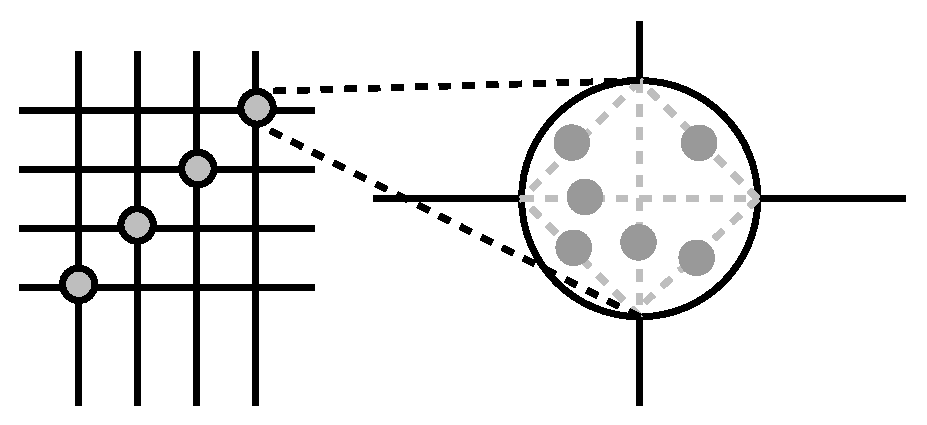
\includegraphics [width=\textwidth]{pictures/cell}
\caption{Схема блока переключения FPGA}
\label{fpga-cell}
\end{figure}

\subsubsection{Задачи, решаемые на FPGA}

В данное время, основные производители FPGA устройств такие как Xilinx и Altera
предлагают свои решения для различных областей рынка, таких как:

\begin{enumerate}
	\item Аэрокосмическая
	\item Оборонная
	\item Автомобильная
	\item Потребительская
	\item Высокопроизводительные вычисления
	\item Хранение данных
	\item Проводные и беспроводные соединения
	\item Автоматизация индустриальных процессов
	\item Медицинская
	\item Широковещательная
\end{enumerate}

Фактически, все эти решения предполагаю использования FPGA в одном из следующих
вариантов:

\begin{enumerate}
  \item Цифровая обработка сигналов(DSP)
  		Раннее почти целиком занятая специальными DSP-процессорами ниша, открывается
  		для FPGA устройств. Увеличение количества блоков, добавление
  		мультпликаторов, повышение общей тактовой частоты, появление готовых решений
  		вкупе с возможностями параллелизма, позволили сравниться, а иногда и превзойти в
  		производительности. 
  \item Дополнительное счётное устройство с аппаратной реализацией под
  		конкретную задачу.
  		FPGA платы зачастую используются как устройства для счёта некоторых задач. С
  		одной стороны программа реализуется аппаратно, что обеспечивает ускорение, с
  		другой стороны дешевизна, малое энергопотребление, большие возможности для
  		параллелизма делают устройства привлекательными. FPGA используются в
  		декодирование видео и аудио потоков, криптографических задачах, для
  		ускорения работы баз данных, обработки финансовых данных. Компании Intel и
  		AMD предлагают готовые HPC решения использующие FPGA в качестве
  		сопроцессоров. Кроме того, FPGA находят применение в научных расчётных
  		задачах(биология, молекулярная физика).
  \item Реализация логики управления для некоторого устройства.
  		FPGA широко используются в различных областях силовой электроники. К
  		примеру, в самолёте Airbus 380 находится по меньшей мере 700 FPGA чипов. 
  		Данное устройство применяется для реализации управления в электроприводах и
  		устройствах с нечёткой логикой. Согласно проведённым исследованиям,
  		добавление логики управления на FPGA чипе для всех электромоторов в США,
  		позволит экономить в год 15 млрд. \$.
  \item Прототипирование.
  		FPGA являются основой текущей мейнстримовой методологии аппаратной
  		верификации ASIC и SoC а также раннего проектирования проектирования
  		программного обеспечения и прошивок. Компания Intel проектировала на системе
  		FPGA кристаллов процессоры Intel Atom и Intel Nehalem. 
\end{enumerate}